\chapter %\chapter[<ToC-title>]{<Title>}
%we add "\hspace{0.95mm}~" 
%to make the headline align on the top of the pages 
[Continuously Generalizing 
Buildings to Built-up Areas\\%\hspace{0.95mm}~\\
by Aggregating and Growing]
{Continuously Generalizing\\ 
	Buildings to Built-up Areas\\
	by Aggregating and Growing}
\label{chap:Bldg}

%appear at the top of the pages
\chaptermark{Continuously Generalizing 
Buildings to Built-up Areas% by Aggregating and Growing
}

Digital multi-scale maps such as Google Maps and OpenStreetMap 
support zooming by displaying maps at different levels. 
This discrete strategy may result in sudden changes, 
which disturb user navigation.
To provide better zooming experience, 
we try to produce a sequence of maps 
with small incremental changes 
from a level to another level.
This process is known as \emph{continuous generalization}.

A way to achieve continuous generalization is to use morphing.
Often, a start map (at a larger-scale) and 
a goal map (at a smaller-scale) 
are used as input, 
then maps at intermediate scales are produced 
while the start map is morphed to the goal map.
In order to morph, correspondences 
between two maps need to be defined.
For example, corresponding points 
between a pair of polylines have been investigated based on 
dynamic programming \citep{Noellenburg2008}, 
Delaunay triangulations and 
binary line generalisation tree \citep{Deng2015},
and simulated annealing \citep{Li2017Annealing}.
From a point to its corresponding point,
a straight-line trajectory is often used to interpolate.
\citet{Peng2013LSA} defined trajectories 
based on least-square adjustment 
in order to obtain more reasonable intermediate-scale polylines.
Using morphing, \citet{Peng2016Admin} continuously generalized 
administrative boundaries based on compatible triangulations. 
When the numbers of line features are different 
on the start and goal maps, 
a continuous selection is required; 
\citet{Chimani2014Eat} proposed to generate a 
removing sequence applicable for road network.
They removed one road at each step
while keeping the remaining roads connected.

These methods are interesting but only work on lines. 
Our problem of building polygon interpolation 
cannot be achieved by similar morphings. 
Regarding the continuous generalization of polygon features,
\citet{Danciger2009} grew polygons during zooming out. 
Their method preserves polygons' 
topology, area-ratios, and relative positions.  
In the case where the goal map is an aggregated version of 
a start land-cover map, 
\citet{Peng2017AStar} computed optimal sequences 
for aggregating land-cover areas.

Buildings are important elements on maps. 
Many methods have been proposed to generalize them 
but not necessarily in a continuous way.
For example, \citet{Haunertwolff2010Building} simplified a set 
of buildings based an integer program.
Their simplification minimizes the number of total edges and 
guarantees that the errors are smaller than 
a user-defined tolerance.
At the same time, their method does not introduce any topological conflict.
\citet{Buchin2011_Simp} simplified buildings based on 
edge-move operations.
Their method preserves orientations of the edges.

When users zoom out on digital maps, 
buildings become smaller and 
the distances between them decrease. 
In addition to simplifying the buildings,
we also need to aggregate them when they become close \cite{Weibel1997}. 
Several methods were proposed 
to aggregate buildings while preserving their shape 
(e.g., right angles);
see \citet{Regnauld2001,RegnauldRevell07,Damen2008}. 
These algorithms can be used as inspirations 
to define a continuous transformation of buildings.

Algorithms were also proposed to create 
built-up areas (that appear on our goal map) from 
individual buildings (that appear on our start map). 
For instance, \citet{Chaudhry2008} identified 
the boundaries of urban settlement 
by calculating `citiness' based on buildings. 
However, this method cannot be adapted 
to provide a continuous transformation 
from buildings to built-up areas.

Finally, some papers directly tackle 
the continuous transformation of buildings 
when scale is reduced. 
\citet{Li2017_Building} morphed between two buildings 
at different scales.
They managed to preserve the orthogonal characteristics of 
buildings, but their algorithm cannot be used in our case 
as our goal map does not contain buildings anymore.
\citet{Touya2017Progressive} 
transformed buildings into built-up areas, 
where they progressively replaced buildings 
by the shape of the blocks to which the buildings belong. 
However, this last algorithm is not continuous enough 
because each iteration directly transforms 
a set of buildings in a block to a polygon 
that covers the whole block. 
As a result, there is no existing solution 
for the continuous generalization of buildings 
into built-up areas.


Our contributions are as follows.
In \sect\ref{sec:Methodology},
we continuously generalize a start map of buildings
(at a larger scale) 
to a goal map of built-up areas (at a smaller scale).
The generalization consists of 
aggregating, growing, and simplifying.
We aggregate the original buildings which will be too close 
at an output scale by adding bridges.
We grow (bridged) original buildings by buffering,
where we use so-called \emph{miter} joins to keep the right 
angles of buildings.
Because of using this kind of joins 
instead of \emph{round} ones,
we have new problems.
We show how to solve these problems.
We also simplify the buildings according to output scales.
Finally, we analyze running time at the end of this section.
We carry out a case study 
and discuss the performances of our method in 
\sect\ref{sec:CaseStudy}.
We conclude this chapter in \sect\ref{sec:Conclusion}.

\section{Methodology}
\label{sec:Methodology}
The input map is our start map.
We denote the scale of the start map by~$1:M_\mathrm{s}$.
We generate the goal map at scale~$1:M_\mathrm{g}$ 
($M_\mathrm{g} > M_\mathrm{s}$) by generalizing the start map. 
We use time~$t\in[0,1]$ to define 
the process of continuous generalization. 
We require that 
the generalization yields exactly the start map when~$t=0$ 
and the goal map when~$t=1$.
The start map should be continuously changed to the goal map 
when~$t$ increases from~$0$ to~$1$.
For the sake of convenience, we define 
\emph{scale denominator}~$M_t= 
M_\mathrm{s} + t \cdot (M_\mathrm{g}-M_\mathrm{s})$.

We carry out the continuous generalization 
by growing the original buildings. 
If some grown buildings become too close at time~$t$,
we aggregate the related original buildings by adding bridges.
We grow the (bridged) original buildings 
by buffering with miter joins.
At any time $t$, the grown buildings 
need to be simplified to look like buildings.
This simplification is carried out in two steps:
the first one is to use dilating and eroding 
to remove ``dents'' and ``bumps''; 
the second step is to remove vertices 
using the algorithm of \citet{ImaiIri1988}.
To make sure that buildings never shrink 
when~$t$ is increasing,
we merge the shape of a building at time~$t$ 
and its shape at the preceding time (before~$t$). 
We clip the buildings using the shape on the goal map to 
ensure that the buildings will not 
grow out of the intended built-up areas.
\fig\ref{fig:Bldg_Framework} shows 
the framework of our method;
we explain the presented operators
in the following subsections.




\begin{figure}[tb]
\centering
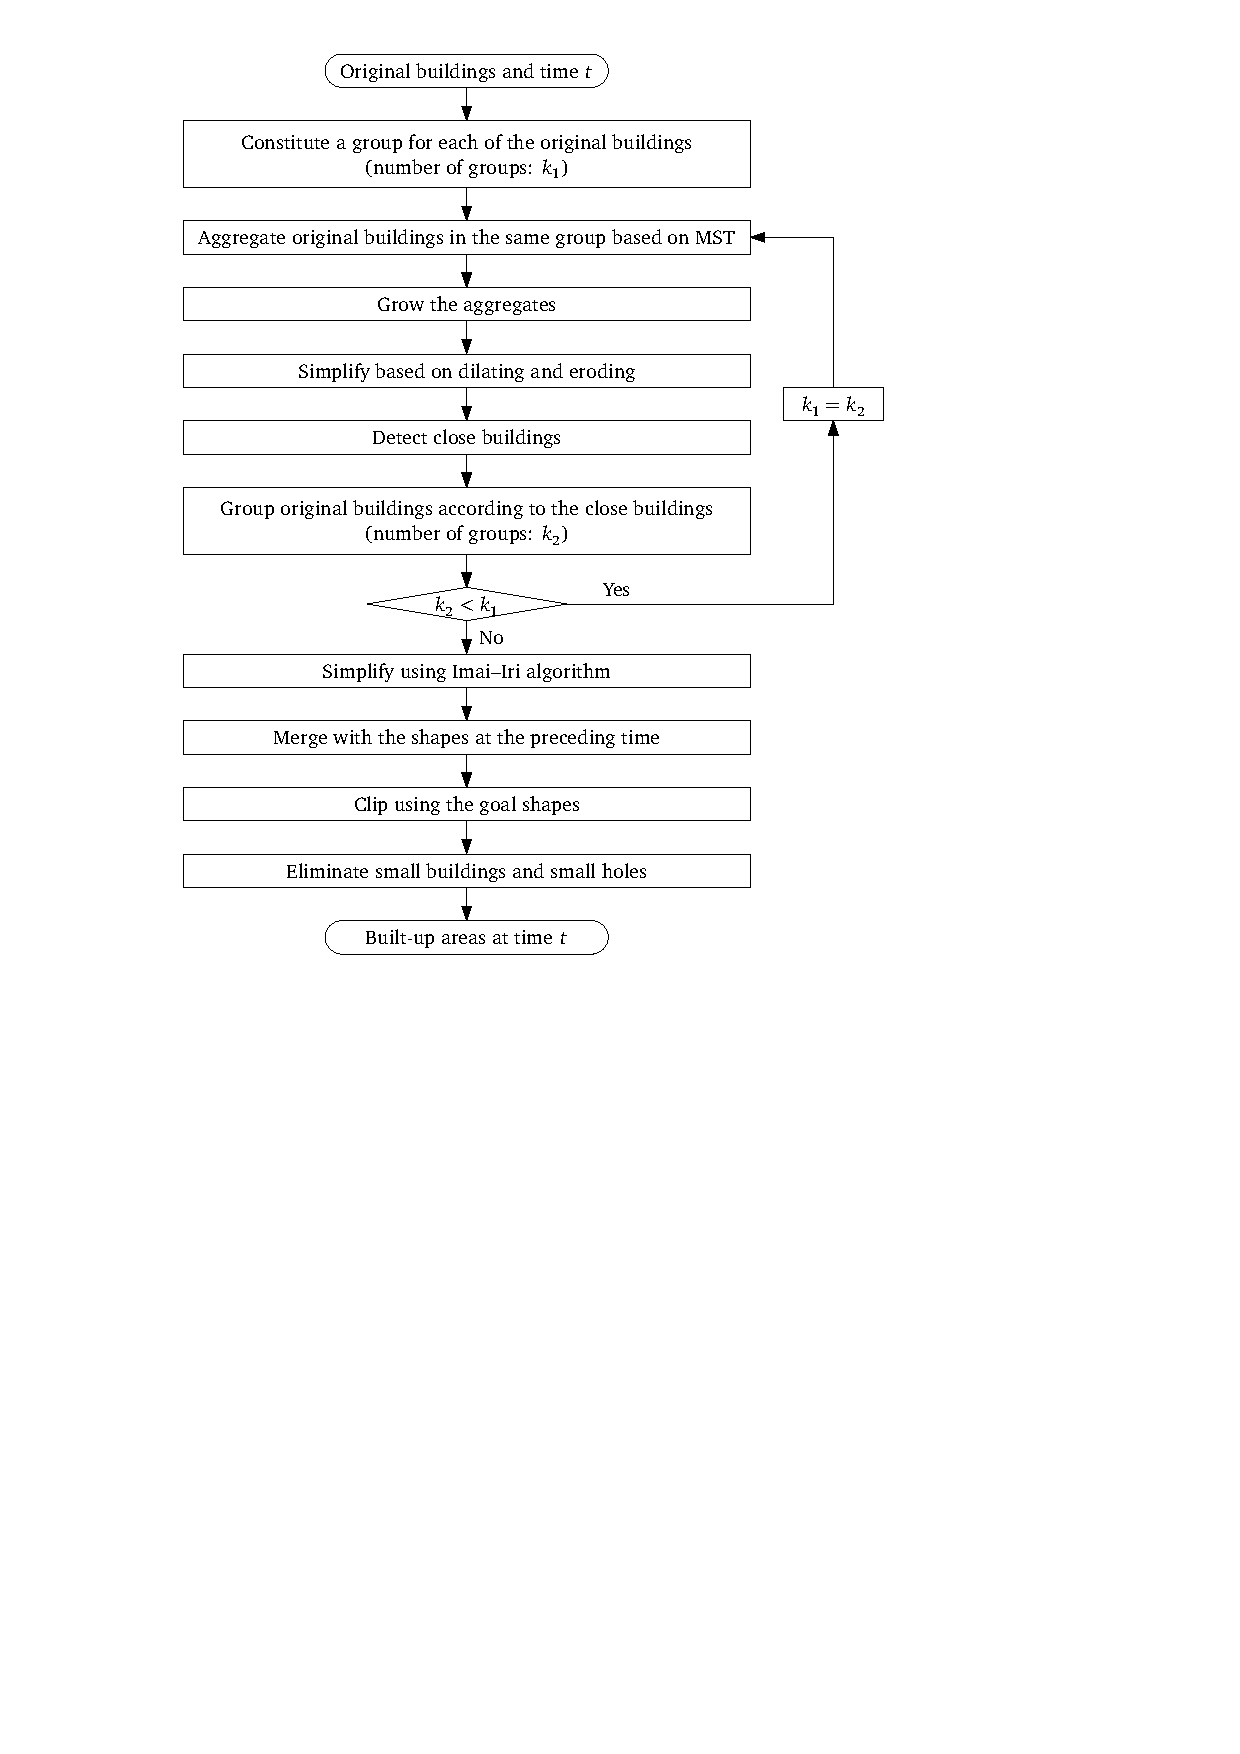
\includegraphics[page=1]{Bldg_Framework}
\caption{The framework of our method.}
\label{fig:Bldg_Framework}
\end{figure}


\subsection{Growing buildings by buffering}
\label{sec:Grow}
We denote by $d_\mathrm{G}$ 
the \emph{growing distance} for the goal map.
At time $t$, the distance is
\begin{equation}
\label{eq:d_Gt}
\dtrm{G} = t \cdot d_\mathrm{G}.
\end{equation}

There are three typical joins when buffering a polygon, i.e.,
round, miter, and square joins
(see \fig\ref{fig:Buffer_ThreeKinds}).
We choose the miter joins to grow buildings in order to
preserve right angles.
If an angle is acute, however, 
an excessively long \emph{spike} will be produced.
This spike may go across other buildings 
(see for example \fig\ref{fig:Buffer_MiterLimits}a).
To avoid this kind of interruptions, 
we require that if the tip of a spike 
is more than $\alpha \dtrm{G} (\alpha \ge 1)$
away from the original vertex, 
then we apply a \emph{square} join
(see \fig\ref{fig:Buffer_MiterLimits}b).
To keep right angles of buildings, 
we must have \emph{miter limit}~$\alpha \geq \sqrt{2}$. 
We set $\alpha  = 1.5$. 
In this case, a square join will be applied 
when an angle is smaller (more acute) than $83.6 \degree$.

\begin{figure}[tb]
\centering
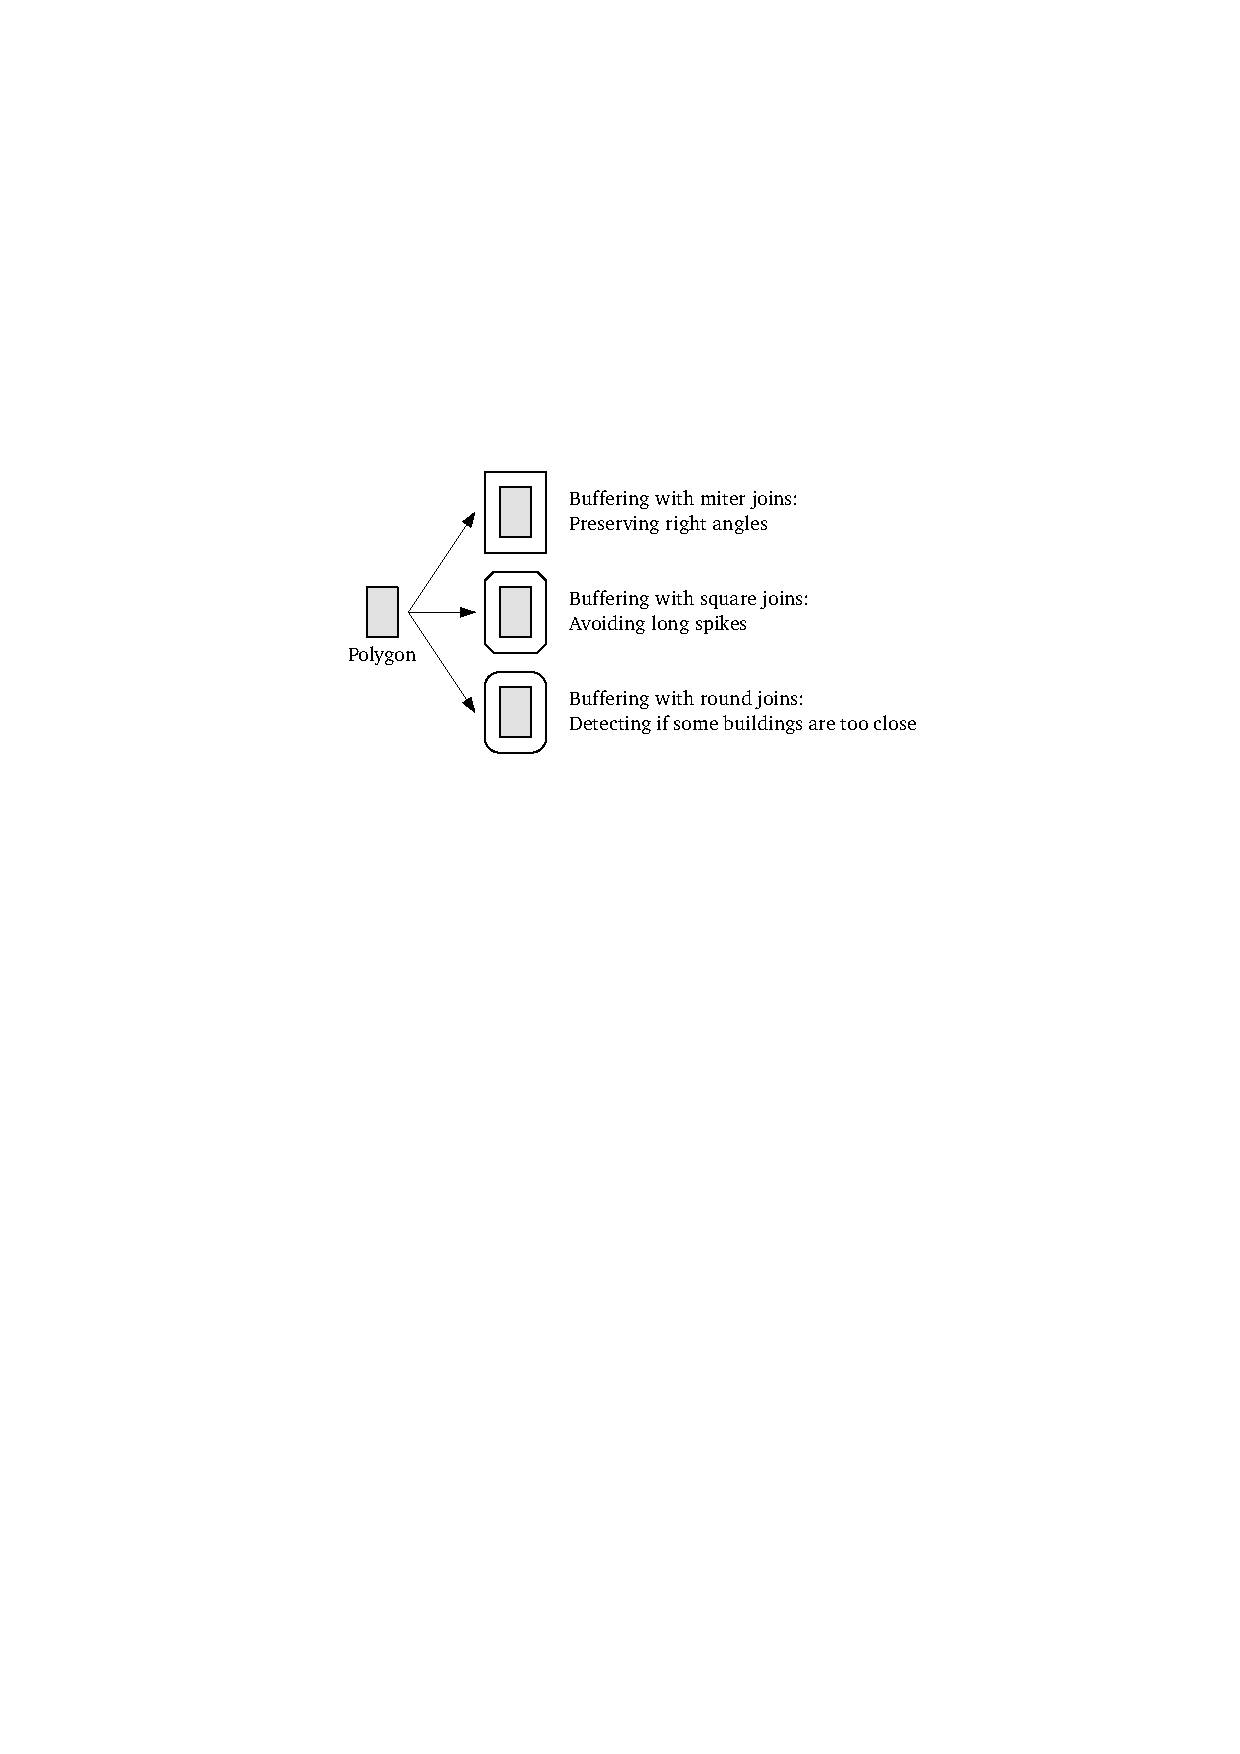
\includegraphics[page=1]{Bldg_Buffering}
\caption{Three ways of buffering a polygon and 
	their applications.}
\label{fig:Buffer_ThreeKinds}
\end{figure}

\begin{figure}[tb]
\centering
\includegraphics[page=2]{Bldg_Buffering}
\caption{Using square joins instead of miter joins to avoid
    long spikes.
}
\label{fig:Buffer_MiterLimits}
\end{figure}




\subsection{Simplifying grown buildings based on dilating and 
eroding}
\label{sec:DilationErosion}
As mentioned earlier, 
methods of simplifying building have already been well studied. \citet{Damen2008} generalized buildings using 
morphological operators.
A drawback of their method is that the orientation of the 
buildings have to be identified.
\citet{Meijers2016} simplified buildings 
using offset curves generated based on straight skeletons.
Our method is similar to \citet{Meijers2016}.
We dilate and erode the buildings to remove dents and 
bumps that can occur when buildings grow
(see \fig\ref{fig:RemoveDentAndBump}).

\begin{figure}[tb]
\centering
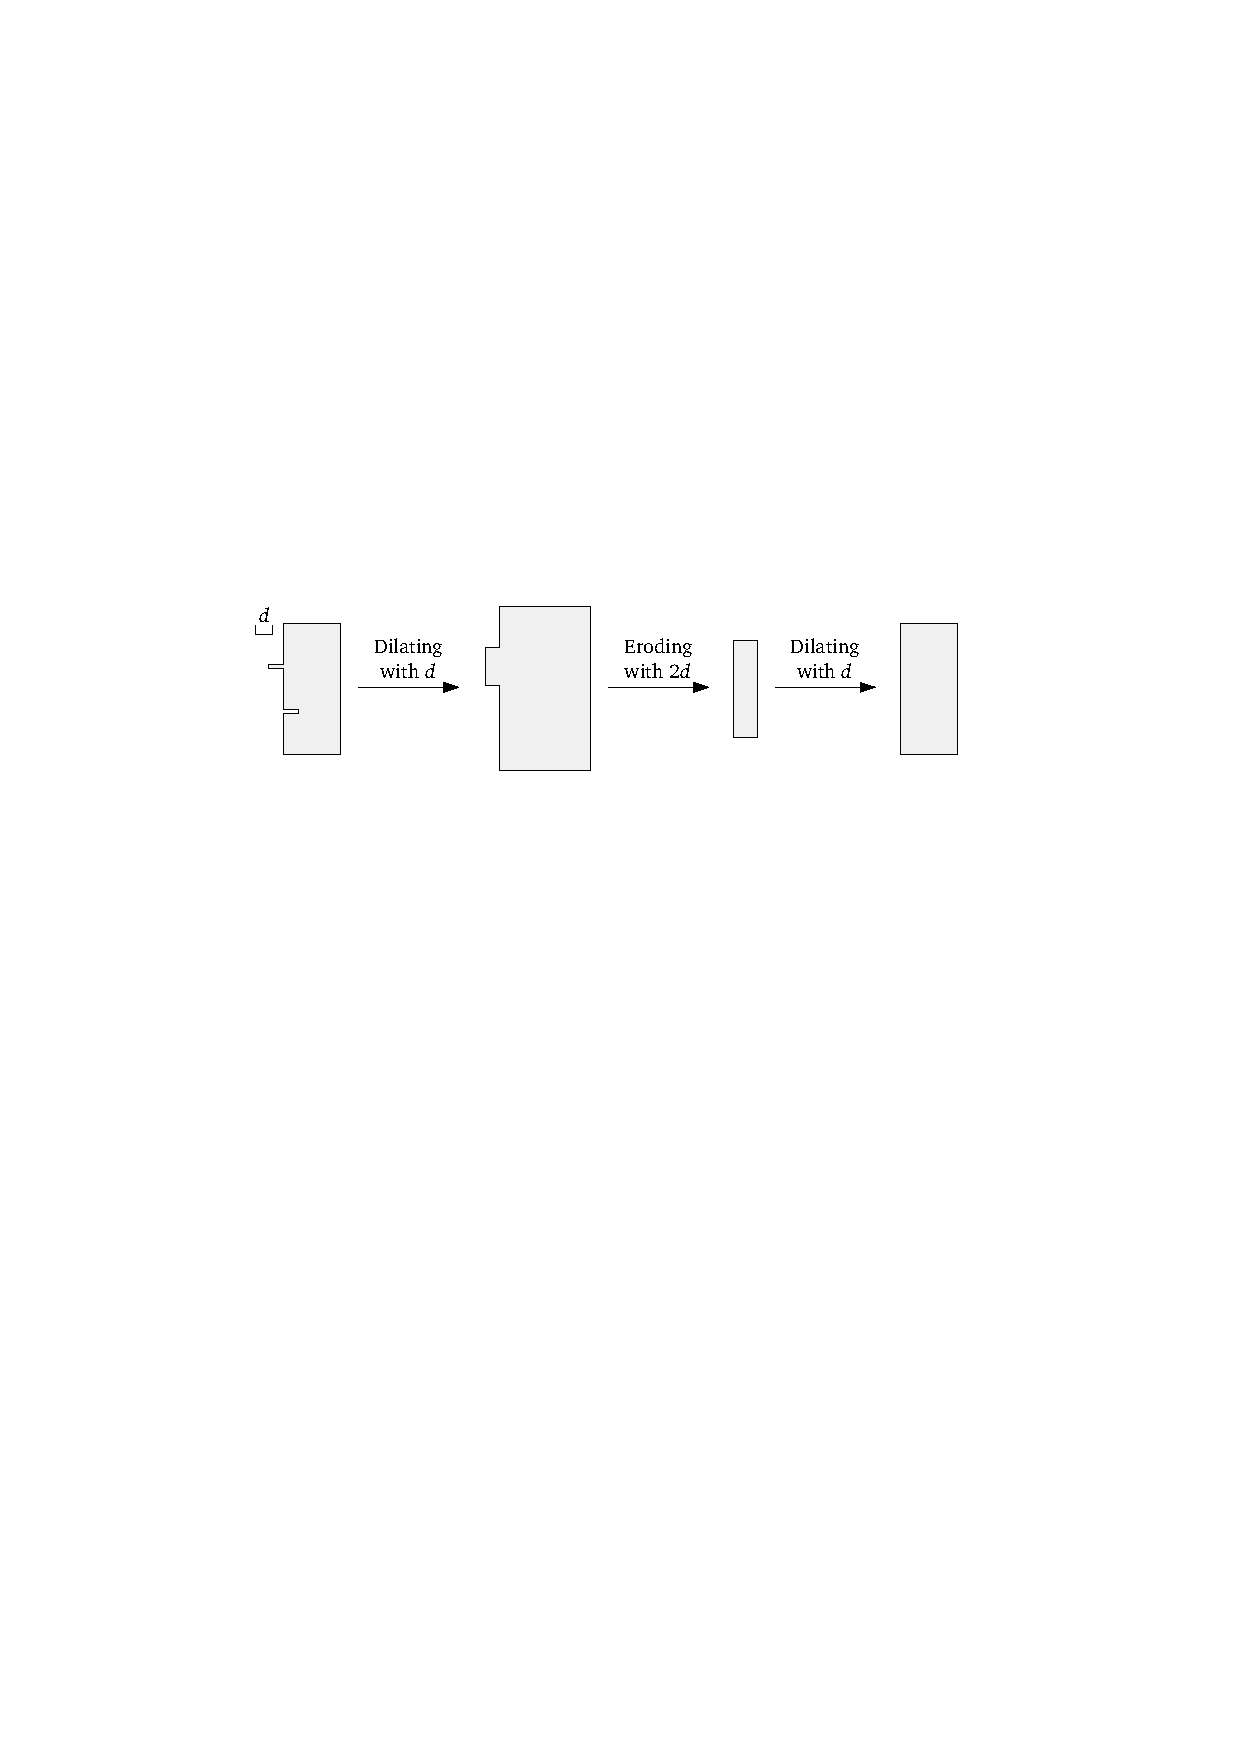
\includegraphics[page=1]{Bldg_DilationErosion}
\caption{Removing dents and bumps 
	by dilating and eroding with distance~$d$.
}
\label{fig:RemoveDentAndBump}
\end{figure}

At time~$t$, we should grow buildings with distance~$\dtrm{G}$.
In order to simplify the grown buildings, 
we further dilate them with distance $\dtrm{D}$ ($\dtrm{D}>0$),
erode with $\dtrm{D}+\dtrm{E} (\dtrm{E}>0)$,
and dilate back with $\dtrm{E}$.
A problem of this process is that 
a building may be split into several parts by eroding
(see \fig\ref{fig:ErosionBreak} for example).
The reason is that 
some parts of a building may be increased (by growing and 
dilating) 
with distance $\dtrm{G}+\dtrm{D}$, 
but can be decreased (by eroding) as much as $\alpha 
(\dtrm{D}+\dtrm{E})$.
If $\dtrm{G}+\dtrm{D} < \alpha (\dtrm{D}+\dtrm{E})$ 
and the building is not thick enough, 
a thin part may disappear
(see \fig\ref{fig:ErosionBreak} when using distance~$d_2$).
In order to avoid this problem, we require that
\[
\dtrm{G} + \dtrm{D} \ge \alpha (\dtrm{D}+\dtrm{E}),
\]
which means
\begin{equation}
\label{eq:d_DtBound}
\dtrm{D} \le \frac{\dtrm{G}-\dtrm{E}}{\alpha - 1}.
\end{equation}

\begin{figure}[tb]
\centering
\includegraphics[page=2]{Bldg_DilationErosion}
\caption{Dilating and eroding a polygon 
	with distances~$d_1$ and~$d_2$, where $d_1 < d_2$.
	The result of using~$d_1$ 
	is the same as the original polygon,
	while the result of using~$d_2$
	become two polygons.
}
\label{fig:ErosionBreak}
\end{figure}

We would like to use $\dtrm{E}=\frac{l}{2} \cdot M_t$ so that
any dents and bumps narrower than $l$ will be removed. 
We set~$l=0.3\,\mathrm{mm}$ on map, 
which was used as a length threshold by, for example, 
\citet{Regnauld2001}.
Unfortunately, distance $\dtrm{G}$ can be arbitrarily small 
according to \eq\ref{eq:d_Gt}, 
but $\dtrm{E}$ is at least $\frac{l}{2} M_\mathrm{s}$. 
When time~$t$ is small, $\dtrm{G}-\dtrm{E} \le 0$, 
which violates \eq\ref{eq:d_DtBound}, where $\dtrm{D}>0$.
To mediate this violation, we set eroding distance
\begin{equation}
\label{eq:d_Et}
\dtrm{E} =t \cdot \frac{l}{2} M_\mathrm{g}.
\end{equation}
%Still, we should make sure that $\dtrm{G}-\dtrm{E} > 0$, which 
%means
%$t \cdot \frac{\lambda}{2}\sqrt{a} (M_\mathrm{g}-M_\mathrm{s})-
%t \cdot \frac{l}{2} M_\mathrm{g} >0$.
Still, we have to make sure that $\dtrm{G}-\dtrm{E} > 0$, which 
means
$t \cdot d_\mathrm{G} - t \cdot \frac{l}{2} M_\mathrm{g} >0$.
As a result, we need to make sure that
\begin{equation}
\label{eq:S_g}
M_\mathrm{g} < \frac{2 d_\mathrm{G}}{l}.
\end{equation}

When we grow a bridged building,
a ``bay'' may appear (see \fig\ref{fig:RemoveBay}b).
We remove such a bay by dilating (see \fig\ref{fig:RemoveBay}c)
and then eroding (see \fig\ref{fig:RemoveBay}d) with distance 
$\dtrm{D}$.
We define the width of a bay as the diameter of the largest 
circle 
that can be placed in the bay.
If the width of a bay is smaller than $2\dtrm{D}$, 
then the bay can be removed by dilating with distance 
$\dtrm{D}$.
We wish to remove bays 
which have widths less than~$2 r_\mathrm{h}$.
Variable~$r_\mathrm{h}= 2\sqrt
{ a_\mathrm{h}/ \pi }$
is the radius of a hole 
which is just large enough to be presented on map.
Following \citet{Chaudhry2008}, 
we set area~$a_\mathrm{h} = 8\,\mathrm{mm}^2$ on map.
Sometimes, our~$\dtrm{D}$ is not large enough to remove a bay 
with width~$r_\mathrm{h}$
because of the limitation from \eq\ref{eq:d_DtBound}.
Therefore, we define
\begin{equation}
\label{eq:d_Dt}
\dtrm{D} =\min (\frac{\dtrm{G}-\dtrm{E}}{\alpha - 1}, 
r_\mathrm{h} M_t) .
\end{equation}


\begin{figure}[tb]
\centering
\includegraphics[page=3]{Bldg_DilationErosion}
\caption{Removing a bay by dilating and eroding.
	(a) An aggregate from adding bridges 
	(see \sect\ref{sec:Aggregate}).
	(b) Growing the aggregate with 
	distance~$\dtrm{G}$,
	where the region marked by the dashed circle is a bay.
	(c) Dilating the grown building with~$\dtrm{D}$.
	(d) Eroding the dilated building with~$\dtrm{D}$.
}
\label{fig:RemoveBay}
\end{figure}


\subsection{Iteratively aggregating close buildings by adding 
bridges}
\label{sec:Aggregate}


We grow each original building and, as illustrated in 
\sect\ref{sec:DilationErosion}, simplify the grown building.
If some buildings become too close after these operations,
we aggregate them by adding bridges
(see for example \fig\ref{fig:GrowAndBridge}).
Following \citet{Stoter2009}, 
we define that two buildings are too close if their distance is 
less than
$\varepsilon= 0.2\,\mathrm{mm}$ on map.
The real separation threshold at time $t$ is
\begin{equation*}
\label{eq:d_epsilont}
d_{\varepsilon, t} = \varepsilon \cdot M_t.
\end{equation*}

\begin{figure}[tb]
\centering
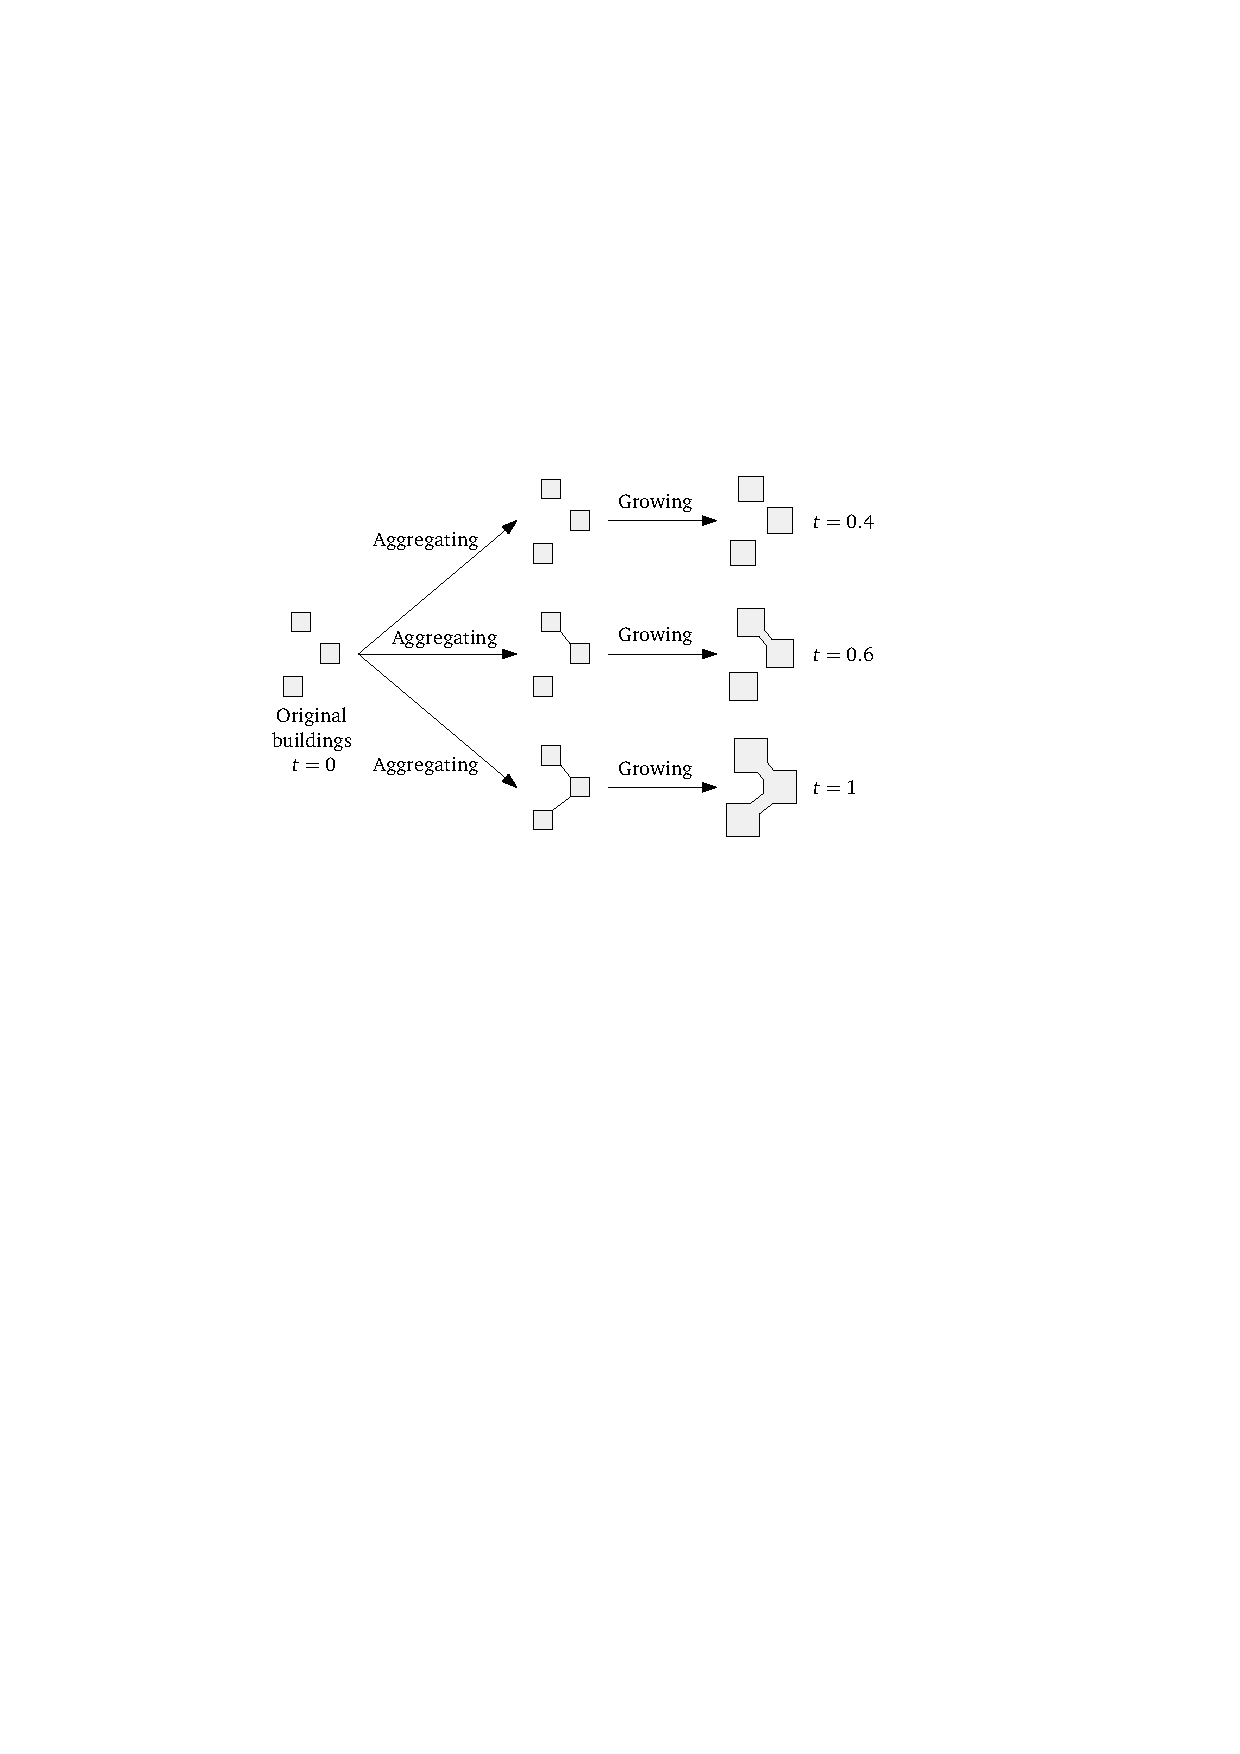
\includegraphics[page=1]{Bldg_Aggregating}
\caption{Aggregating original buildings 
	that will become too close at a certain time 
	by adding bridges;
	then, growing the bridged buildings.}
\label{fig:GrowAndBridge}
\end{figure}

Our way of detecting close buildings is simple.
We buffer buildings with distance 
$\left. d_{\varepsilon,t}\middle/2 \right.$
using round joins
(see \fig\ref{fig:Buffer_ThreeKinds});
then, we merge the buffers that intersect with each other.
On this basis, 
the original buildings intersecting with the same merged buffer 
are identified as a group of close buildings.
For each pair of the original buildings in the same group,
we connect them by adding a line segment 
linking the pair of nearest points.
There can be many line segments, 
and they may cross each other or even intersect with buildings.
To make the topology simple, 
we select only some of the line segments as \emph{bridges}.  
If we consider each building as a node and 
each line segment as an edge, 
then we have a graph.
Using the algorithm of \citet{Prim1957}, 
we find a minimum spanning tree (MST) in the graph,
using the lengths of the line segments as the weights.
As a result, we use the line segments 
that corresponds to the edges in the MST as bridges.
We aggregate the group of original buildings 
by adding these bridges.

Aggregated and grown buildings may become too close 
because of the additional bridges,
so we have to iterate the aggregation process.
\fig\ref{fig:BridgeMoreBuilding} shows such an example.
We grow and buffer buildings~$p$, $q$, and~$r$.
As the buffers of~$q$ and~$r$ intersect
(see \fig\ref{fig:BridgeMoreBuilding}c),
we aggregate buildings~$q$ and~$r$ by adding a bridge
(see \fig\ref{fig:BridgeMoreBuilding}d).
There are two buildings left in 
\fig\ref{fig:BridgeMoreBuilding}d:
an original one and an aggregate.
We then grow and buffer the two buildings in 
\fig\ref{fig:BridgeMoreBuilding}d, 
the buffer of building~$p$ intersects with
the buffer of the bridge of buildings~$q$ and~$r$
(see \fig\ref{fig:BridgeMoreBuilding}f).
Finally, we aggregate building~$p$ with bridged~$q$ and~$r$
(see \fig\ref{fig:BridgeMoreBuilding}g), 
and there is only one building left in 
\fig\ref{fig:BridgeMoreBuilding}g.
Then, we grow and buffer again 
to get the final shape of the group.
As the number of buildings 
does not decrease from \fig\ref{fig:BridgeMoreBuilding}g
to \fig\ref{fig:BridgeMoreBuilding}i,
we stop the iteration.

When buildings are grown and aggregated iteratively, 
bridges have been added. 
These bridges have a width of~$2\dtrm{G}$ at time~$t$.
This setting guarantees that no bridge is thin when~$t=1$.
As we aggregated all the buildings that will become too close, 
all the separation distances 
between each pair of buildings (or aggregates) 
are larger than distance~$d_{\varepsilon, t}$.
Specifically, if a group of buildings 
will be aggregated at time~$t=1$, 
we say that these buildings are in the same \emph{goal group}. 

\begin{figure}[tb]
\centering
\includegraphics[page=2]{Bldg_Aggregating}
\caption{Iteratively aggregating close buildings 
	by adding bridges.
}
\label{fig:BridgeMoreBuilding}
\end{figure}

\subsection{Simplifying buildings using the Imai--Iri algorithm}
\label{sec:ImaiIri}

When the scale is decreasing ($M_t$ increasing), 
we should remove more and more details. 
So, we simplify the (aggregated) grown buildings
using the Imai--Iri algorithm \citep{ImaiIri1988}.
First, this algorithm finds 
all the valid shortcuts of a polyline.
A shortcut is valid for a segment 
if the distance between the segment and the shortcut 
is at most a specified value
(see \fig\ref{fig:ImaiIri_Shortcut}).
We set the value also as~$l=0.3\,\mathrm{mm}$ on map
(see \sect\ref{sec:DilationErosion}). 
That is, at time~$t$, the distance threshold is
\begin{equation}
\label{eq:d_lt}
d_{l,t}= l \cdot M_t.
\end{equation}
Second, the algorithm finds a sequence of valid shortcuts
using breadth-first search.
The sequence of valid shortcuts 
is an approximation of the polyline 
and has the least number of line segments, 
with error smaller than~$d_{l,t}$.

\begin{figure}[tb]
\centering
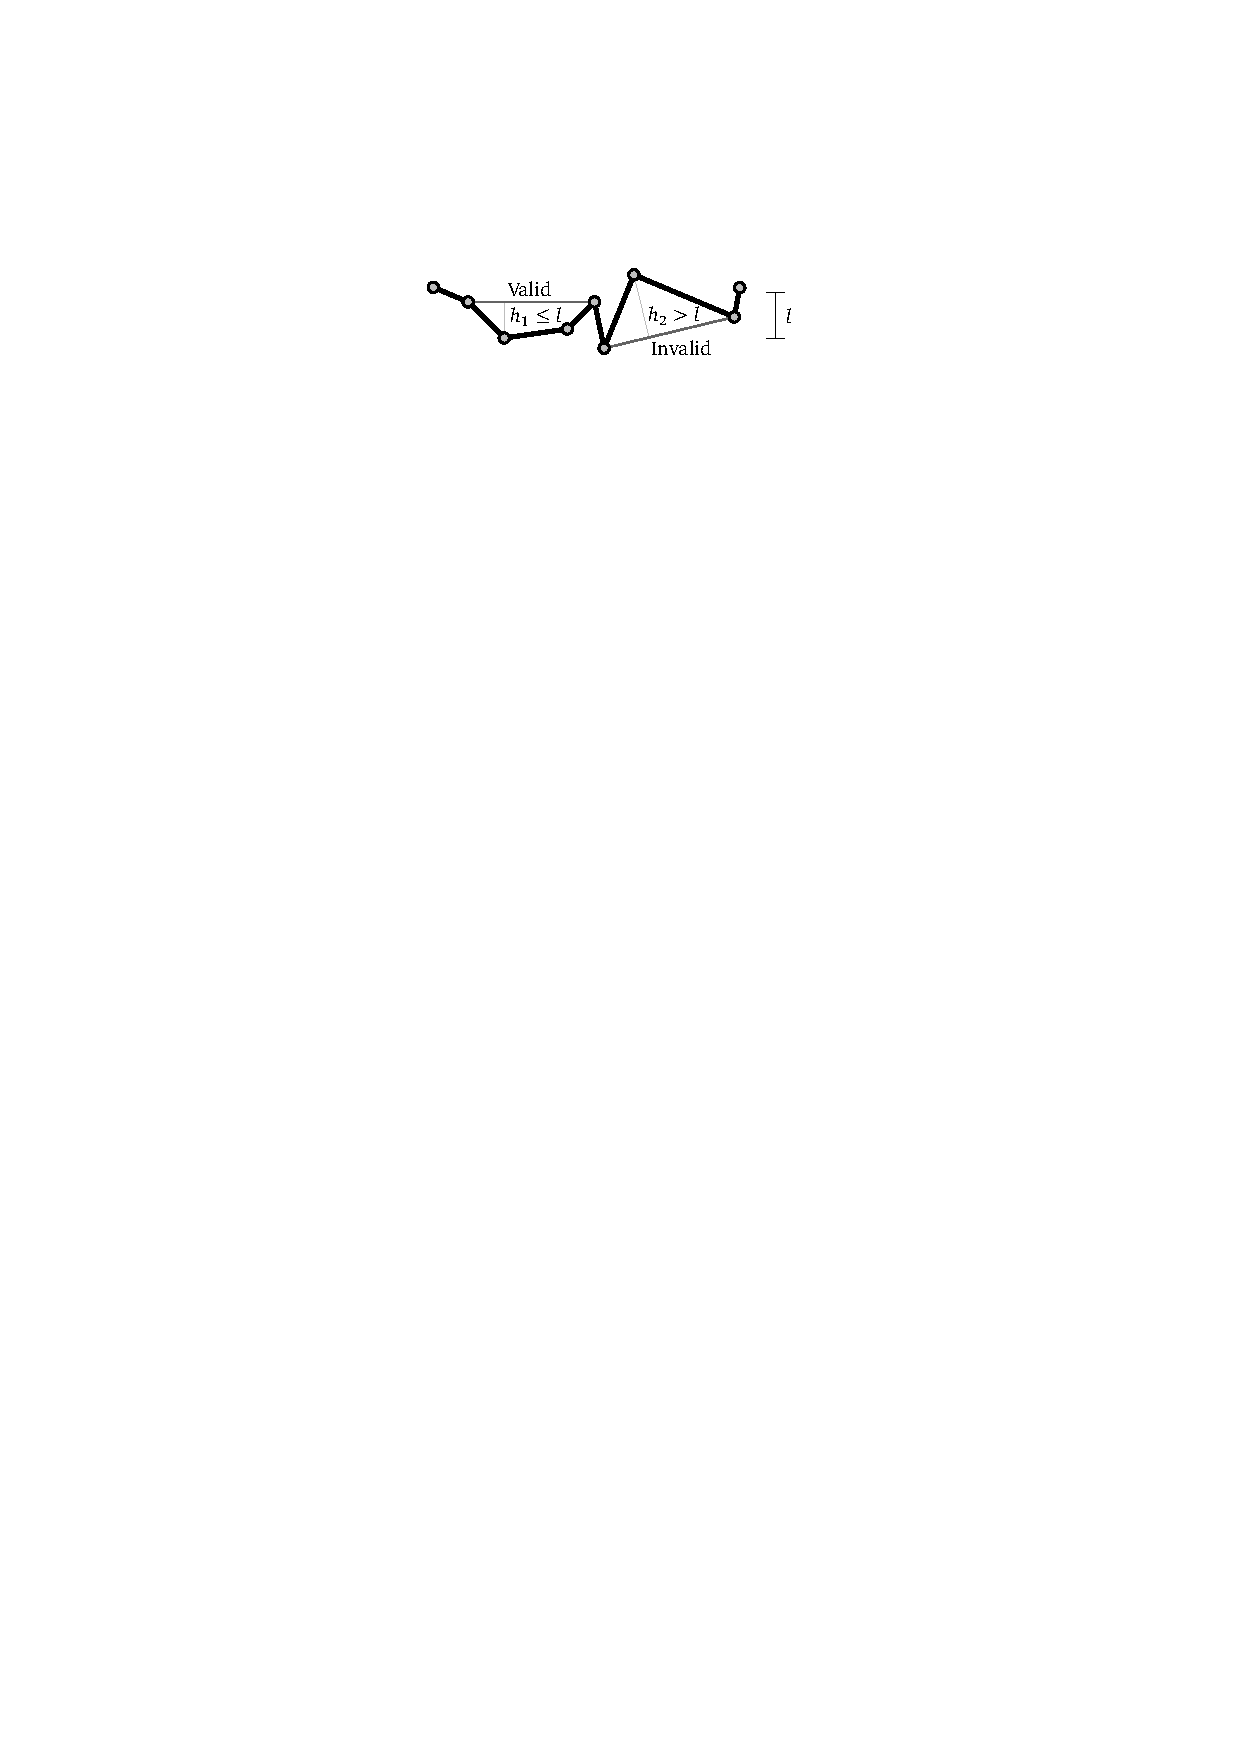
\includegraphics[page=1]{Bldg_Shrinking}
\caption{Valid and invalid shortcuts 
	for the Imai--Iri algorithm.
	Parameter~$l$ is the tolerance for errors.}
\label{fig:ImaiIri_Shortcut}
\end{figure}

In order to adapt the Imai--Iri algorithm to our problem,
we add two more constraints for a shortcut to be valid. 
One is that a shortcut must be 
completely inside the grown building.
If a shortcut is outside,
we may not be able to arrive at the shortcut by growing.
The other constraint is that 
a shortcut is not allowed to intersect with
the resulting building at the preceding time frame.
We add this constraint 
to avoid the building to shrink.

The classical way of simplifying
a polyline or a polygon is using 
the Douglas--Peucker algorithm \citep{Douglas1973}. 
However, it cannot simplify the shapes enough in our case.
This is why we choose the Imai--Iri algorithm.


%
%
%\subsection{Generating the goal shapes of buildings}
%\label{sec:Goal}
%To generate the goal shapes of buildings, we set time $t=1$.
%We aggregate original buildings (see \sect\ref{sec:Aggregate}).
%Then we grow (see \sect\ref{sec:Grow}) 
%and simplify 
%(see \sects\ref{sec:DilationErosion} and~\ref{sec:ImaiIri}) 
%the 
%grown 
%buildings.
%See for example \fig\ref{fig:GrowAndBridge}, 
%the building at time $t=1$ is the goal shape of the three 
%original buildings.
%
%


\subsection{Generating buildings on intermediate-scale maps}
\label{sec:Unite}

Both the eroding and the line simplification 
may result in a building to be shrunk.
\fig\ref{fig:Shrink_Erosion} and 
\fig\ref{fig:Shrink_Simplification} show such 
examples, respectively.
To avoid these kinds of shrinking,
for a building, we merge its shape at time $t$ 
and its shape at the preceding time (before~$t$). 
For example, we generate a sequence of~$10$ maps,
which means~$t \in \{0.1, 0.2, \dots, 1\}$.
\fig\ref{fig:Shrink_Erosion}c shows the result at~$t=0.6$.
In \fig\ref{fig:Shrink_Erosion}f, 
the darker gray piece is included in the result at~$t=0.6$
but not in the result at~$t=0.7$.
In other words, the result at~$t=0.7$ 
shrinks at the darker gray part.
To prevent this shrinking, 
we merge the result at~$t=0.7$ with 
the result at the preceding time, i.e., $t=0.6$.
The merged result is shown in \fig\ref{fig:Shrink_Uniting}a.
Similarly, \fig\ref{fig:Shrink_Uniting}b shows the merged 
result of buildings 
in \fig\ref{fig:Shrink_Simplification}c 
and~\fig\ref{fig:Shrink_Simplification}h.
This merge also avoids bridges' shrinking;
\fig\ref{fig:BridgeDisappearing} shows such an example.

\begin{figure}[tb]
\centering
\includegraphics[page=2]{Bldg_Shrinking}
\caption{A building shrinks because of dilating and eroding, 
	where~$t_1=0.6$ and~$t_2=0.7$.
	The gray polygons in~(a) and~(d) 
	represent the original building.
	The transparent polygon in~(a) is from 
	growing and dilating the original building with 
	distances~$\dtrm[1]{G}$ and~$\dtrm[1]{D}$.
	The transparent polygon in~(d) is obtained analogously
	as in~(a).
	The darker gray piece in~(f) shows 
	the part which is included in the polygon of~(c) 
	but not in the polygon of~(f).
}
\label{fig:Shrink_Erosion}
\end{figure}


\begin{figure}[tb]
\centering
\includegraphics[page=3]{Bldg_Shrinking}
\caption{A building shrinks because of line simplification, 
	where~$t_1=0.7$ and~$t_2=0.8$.
	The gray polygons in~(a) and~(e) 
	represent the original building.
	The transparent polygon in~(a) is from 
	growing and dilating the original building with 
	distances~$\dtrm[1]{G}$ and~$\dtrm[1]{D}$.
	The transparent polygon in~(e) is obtained 
    analogously as in~(a).
	Note that distances~$d_{l,t_1}<d_{l,t_2}$ 
	(see \eq\ref{eq:d_lt});
	this is why the Imai--Iri algorithm does not 
	remove any vertex of the polygon in~(c)
	but removes two vertices of the polygon in~(g).
	The darker gray pieces in~(h) are 
	the parts which are included in the polygon of~(d) 
	but not in the polygon of~(h).
}
\label{fig:Shrink_Simplification}
\end{figure}

\begin{figure}[tb]
\centering
\includegraphics[page=4]{Bldg_Shrinking}
\caption{Merging a polygon with the polygon 
	at the preceding time.
	(a) Merging the transparent polygons in 
	\figs\ref{fig:Shrink_Erosion}c and~\ref{fig:Shrink_Erosion}f.
	(b) Merging the transparent polygons in 
	\figs\ref{fig:Shrink_Simplification}d 
    and~\ref{fig:Shrink_Simplification}h.
}
\label{fig:Shrink_Uniting}
\end{figure}

\begin{figure}[tb]
\centering
\includegraphics[page=5]{Bldg_Shrinking}
\caption{Avoiding shrinking resulted by moved bridges,
	where~$t_1=0.5$ and~$t_2=0.6$.
	(a) Original buildings.
	(b) Growing buildings with distance~$\dtrm[1]{G}$ and 
	dilating with~$d_{\varepsilon,t_1}/2$;
	buildings~$p$ and~$q$ are identified as in the same group.
	(c) Aggregating~$p$ and~$q$	by adding a bridge.
	(d) Growing the (bridged) buildings in (c)
	with distance~$\dtrm[1]{G}$.
	(e) Growing original buildings with 
	distance~$\dtrm[2]{G}$ and 
	dilating with~$d_{\varepsilon,t_2}/2$;
	all the three buildings are in the same group.
	(f) Aggregating	by adding bridges according to the MST.
	(g) Growing the bridged building in~(f)
	with distance~$\dtrm[2]{G}$. 
	The bridge in~(d) shrinks comparing to~(g).
	(h) Avoiding this shrinking at time~$t_2$ 
	by merging buildings in~(d) and~(g).
}
\label{fig:BridgeDisappearing}
\end{figure}

%\begin{figure}[tb]
%	\centering
%	
\includegraphics{Bldg_NearestPoints}
%	\caption{The nearest points between a pair of buildings	
%		change because of growing. 
%		The two squares and the two circles respectively mark
%		the nearest points before and after growing.
%	}
%	\label{fig:NearestPoints}
%\end{figure}

Added to this shrinking problem, 
a building aggregate on an intermediate map should never leave
the goal shape of the aggregated building. 
Otherwise, the building will need to shrink 
to achieve the goal shape.
To avoid shrinking, 
we clip the building using the goal shape 
and remove the parts outside.


\subsection{Eliminating small buildings and small holes}
\label{sec:Eliminate}
Following the previous steps may result in 
some small isolated building aggregates.
We should remove these small aggregates during
the continuous generalization 
because they become too small to be visible at some point.
Therefore, we eliminate a building aggregate if its area is 
smaller than a threshold.
Following \citet{Stoter2009,Chaudhry2008}, 
we set this threshold to~$a=0.16\,\mathrm{mm}^2$ on map.
The real threshold at time~$t$ is
\[
a_t=a\cdot M_t^2.
\]
For the buildings in the same goal group 
(see the definition in \sect\ref{sec:Aggregate}),
we consider the total area of all the buildings at time $t$, 
instead of considering each building individually.

As mentioned in \sect\ref{sec:DilationErosion}, 
we remove holes that have area less than 
$a_\mathrm{h} = 8\,\mathrm{mm}^2$ on map.
The real area threshold for a hole at time $t$ is
\[
a_{\mathrm{h},t}=a_\mathrm{h}\cdot M_t^2.
\]

\subsection{Running time}
Suppose that our input has $n$ edges in total.
Operations like growing, dilating, 
eroding, merging, and clipping 
cost time~$O(n^2)$; see \citet{Greiner1998Clipping,Palfrader2015}.
We iteratively aggregate in \sect\ref{sec:Aggregate}.
In the worst case, we need to repeat $O(n)$ times,
which increases our running time to $O(n^3)$.
It is unlikely that 
we need to repeat the aggregation more than twice, though.
Simplifying polygons using the Imai--Iri algorithm 
takes time~$O(n^3)$.
The improved version of the Imai--Iri algorithm by 
\citet{Chan1996} does not help in our case
because we have more constraints when simplifying
(see \sect\ref{sec:ImaiIri}).
As a result, the running time of our method is in~$O(n^3)$.


\section{Case Study}
\label{sec:CaseStudy}
We have implemented our method based on
C\# (Microsoft Visual Studio 2015) and ArcObjects SDK 10.4.1. 
The code is available in open source on Github\footnote{\url
{https://github.com/IGNF/ContinuousGeneralisation}}.
The offsetting function and clipping function 
are available from library \textsc{Clipper} 
of \citet{Johnson2014}, 
which is based on the clipping algorithm 
of \citet{Vatti1992Clip}.
The offsetting function is used for the buffering, dilating, 
eroding, and merging operations.
We ran our case study under~64-bit 
Windows~7 on a~$3.3\,$GHz dual core CPU with~$8\,$GB RAM.
We measured processing time by the built-in C\# class 
\emph{Stopwatch}.
Our testing data is extracted from a dataset produced 
by the French Mapping Agency (IGN);
see \fig\ref{fig:Data}.
The data is at scale~$1:15{,}000$, 
which means~$M_\mathrm{s}=15{,}000$.
It represents the buildings of four towns, 
i.e., Aussevielle, Denguin,  Poey-de-Lescar, and Siros, 
in the Pyr\'en\'ees-Atlantiques county, south-western France.
IGN also stores a dataset at scale~$1:50{,}000$.
This dataset was obtained mostly
from the data at scale~$1:15{,}000$ 
by buffering with distance~$25\,\mathrm{m}$,
where sometimes distance~$50\,\mathrm{m}$ was also used
in order to identify towns.
A restriction for the town from \citet{Boffet2000} is that 
the longest edge in an MST of the buildings 
should be shorter than~$100\,\mathrm{m}$.

\begin{figure}[tb]
\centering
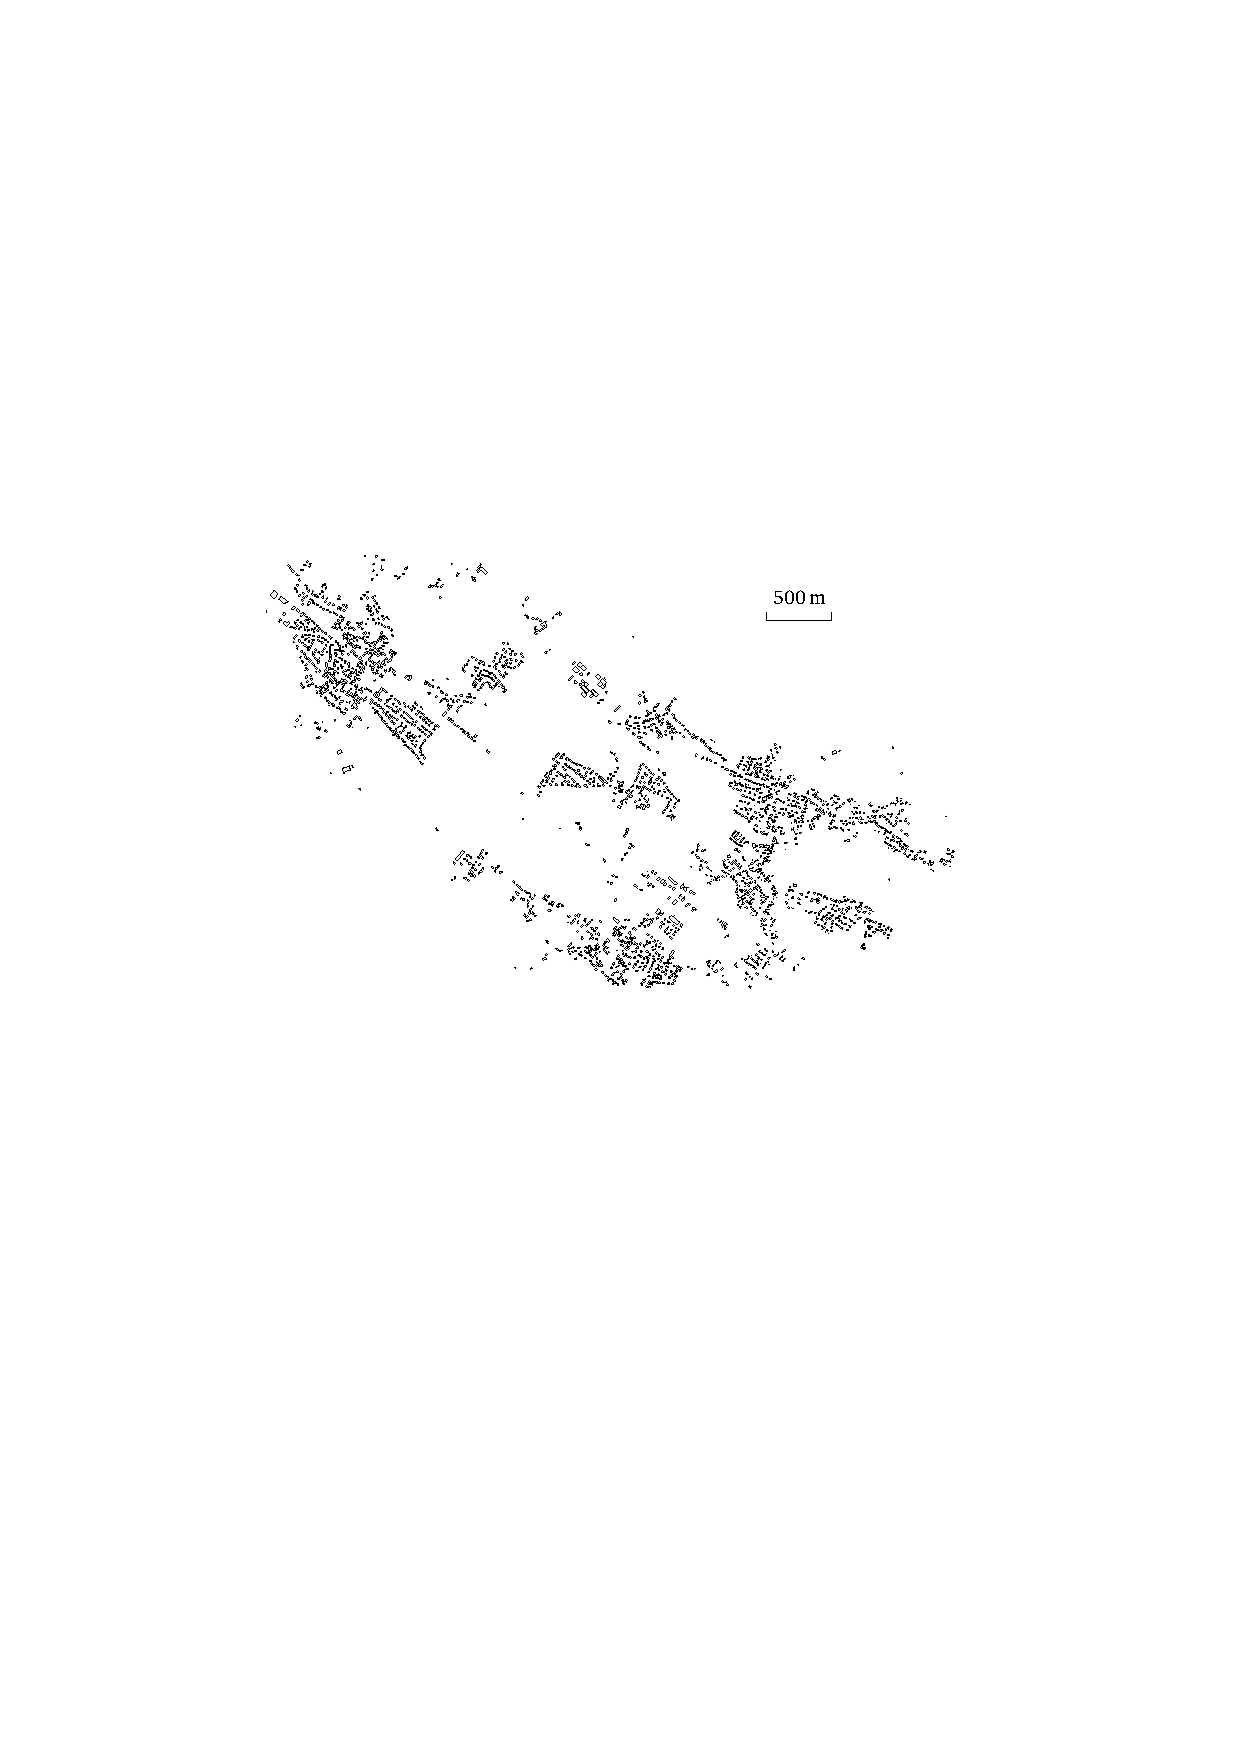
\includegraphics[page=1]{Bldg_CaseStudy_DataAndResults}
\caption{Data for our case study, at scale~$1:15{,}000$.
	There are $2{,}590$ buildings, 
	which in total have $19{,}255$ edges and have area
	$448{,}802.3\,\mathrm{m}^2$.}
\label{fig:Data}
\end{figure}

We set our goal scale to~$1:50{,}000$, 
which means scale denominator~$M_\mathrm{g}=50{,}000$,
and growing distance~$d_\mathrm{G}=25\,\mathrm{m}$
so that we can compare our result with the existing data.
Also, this setting makes \eq\ref{eq:S_g} hold, 
where error tolerance~$l=0.3\,\mathrm{mm}$.
In \eq\ref{eq:d_Dt}, the first part is always smaller than 
the second part because of our settings.
As a result, dilating distance~$\dtrm{D}=t\cdot 35\,\mathrm{m}$, 
where eroding distance~$\dtrm{E}=t\cdot 7.5\,\mathrm{m}$ 
according to \eq\ref{eq:d_Et} and miter limit~$\alpha=1.5$.

Our program took~$93.6\,\mathrm{s}$ 
to compute the goal shapes of the built-up areas.
The~$56$ built-up areas have~$2{,}095$ edges before line 
simplification.
Using the Imai--Iri algorithm, we have~$1{,}102$ edges left.
In comparison, there are~$1{,}597$ edges left 
when we simplified using the Douglas--Peucker algorithm.

\fig\ref{fig:Bldg_GoalShape} shows 
the bridged original buildings as well as the goal shapes.
We produced a sequence of~$10$ maps,
i.e.,~$t \in \{0.1, 0.2, \dots, 1\}$.
This production cost~$668.2\,\mathrm{s}$ in total.
We show such a sequence of maps in 
\fig\ref{fig:ContinuousGeneralization} for 
marked region~$R_1$ in \fig\ref{fig:Bldg_GoalShape}.
The sequence of maps grows continuously, and 
the intermediate results well reflect 
the pattern of the original buildings.
%
Unfortunately, our method produced 
lengthy building aggregates, 
which may annoy users.
Some examples can be found in
\fig\ref{fig:Bldg_Lengthy} when time~$t=0.3$.
To avoid this problem, we could restrict the number of nodes
when we group buildings based on an MST.
Using this restriction, however, 
we will not be able to guarantee that 
the distance between any two (aggregated) buildings 
is larger than distance threshold~$d_{l,t}$
(see \eq\ref{eq:d_lt}).

We counted the numbers of buildings in our results
and compared them to the numbers calculated by
the radical law of \citet{Topfer1966}; 
see \fig\ref{fig:NumberOfBuildings}.
We have exaggerated-area symbols; 
so we use~$C_\mathrm{b3}$ and~$C_\mathrm{z3}$ 
for \eq2 of \citet{Topfer1966}.
As a result, we computed the numbers according to
\begin{equation}
\label{eq:n_t}
n_t=n_\mathrm{s}\left( \frac{M_\mathrm{s}}{M_t}\right) ^2,
\end{equation}
where~$n_s=2{,}590$ is the number of buildings on start map
and~$n_t$ is the number of buildings on the map at scale~$1:M_t$.
\eq\ref{eq:n_t} is intuitive because 
it demonstrates that the number of buildings in a 
unit area on map should be fixed.
According to \fig\ref{fig:NumberOfBuildings}, 
our numbers decrease faster than 
the numbers computed by the radical law.
Still, the radical law seems to agree with our results.


\begin{figure*}[tb]
\centering
\includegraphics[page=2]{Bldg_CaseStudy_DataAndResults}
\caption{Bridged original buildings and
	goal shapes (darker polygons),
	without eliminating small buildings and holes, 
	where the goal shapes are for scale~$1:50{,}000$.
	There are~$56$ goal shapes, which have~$1{,}135$ 
	edges in total.
}
\label{fig:Bldg_GoalShape}
\end{figure*}



\begin{figure*}[tb]
\centering
\includegraphics[page=4]{Bldg_CaseStudy_DataAndResults}
\caption{A sequence of maps 
	at time~$t \in \{0, 0.1, 0.2, \dots, 1\}$ 
	of marked region~$R_1$
	in \fig\ref{fig:Bldg_GoalShape}.
}
\label{fig:ContinuousGeneralization}
\end{figure*}

\begin{figure*}[tb]
\centering
\includegraphics[page=5]{Bldg_CaseStudy_DataAndResults}
\caption{Some intermediate-scale results of  
    marked region~$R_2$ in \fig\ref{fig:Bldg_GoalShape}.
    When time~$t=0.3$, there are some lengthy aggregates.
}
\label{fig:Bldg_Lengthy}
\end{figure*}

\begin{figure}[tb]
\centering
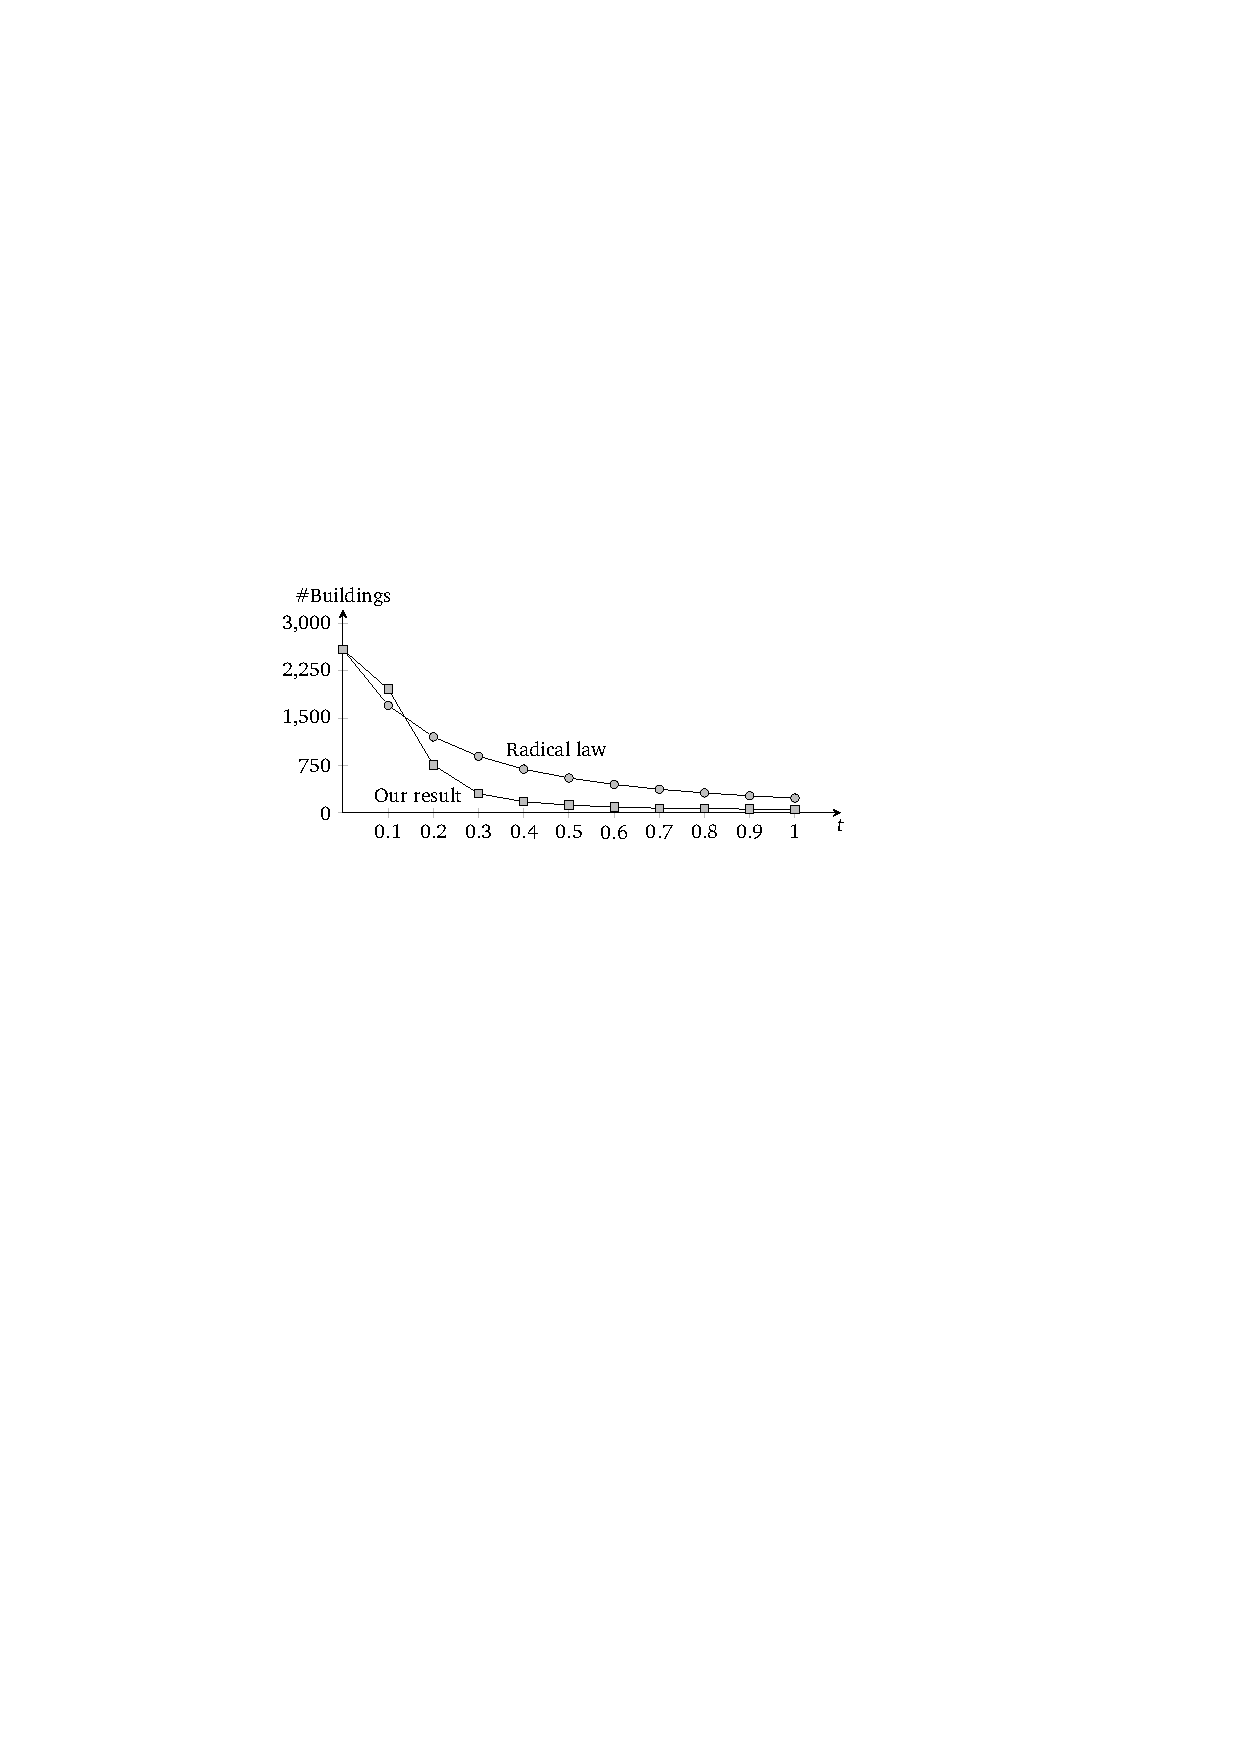
\includegraphics[page=1]{Bldg_CaseStudy_ResultsPlot}
\caption{A comparison of the numbers of buildings 
	between our result and the radical law.}
\label{fig:NumberOfBuildings}
\end{figure}

We also compared the areas on map of our results 
with the areas computed by the radical law of \citet{Topfer1966}.
Our data, at scale~$1:15{,}000$, 
has area~$448{,}802.3\,\mathrm{m}^2$,
which is~$1{,}994.7\,\mathrm{mm}^2$ on map.
The radical law concerns about the number of 
objects, so we slightly abuse the law.
In \eq\ref{eq:n_t}, we replace the number with area and have
$$
A_t=A_\mathrm{s}\left( \frac{M_\mathrm{s}}{M_t}\right) ^2.
$$
The comparison is shown in \fig\ref{fig:AreaOfBuildings}.
The area on map of our results increases 
from time~$t=0$ to time~$t=0.4$. 
The reason is that 
there are many bridges appearing during this period.
Comparing the two curves in \fig\ref{fig:AreaOfBuildings},
we see a disagreement between
the radical law and our results.

\begin{figure}[tb]
\centering
\includegraphics[page=2]{Bldg_CaseStudy_ResultsPlot}
\caption{A comparison of the total area on map of buildings 
	between our result and the radical law.}
\label{fig:AreaOfBuildings}
\end{figure}

In \fig\ref{fig:ExperimentalComparison},
we show our built-up areas at time~$t=1$ (dark polygons)
and the data at scale~$1:50{,}000$ 
from IGN (transparent polygons).
No small building was removed in
our result or the IGN data.
The boundaries of our built-up areas 
are more straight than that of the IGN data. 
We have~$1{,}135$ edges, 
while the IGN data has~$4{,}968$ edges.
From this perspective, our result is 
more reasonable than the existing data.
A questionnaire, however, is needed to 
make a more convincing comparison.

\begin{figure*}[tb]
\centering
\includegraphics[page=3]{Bldg_CaseStudy_DataAndResults}
\caption{A comparison of our built-up areas at time~$t=1$
	and the data from IGN
	at scale~$1:50{,}000$ (transparent polygons).
	Some built-up areas from IGN are split 
	because of streets' crossing.
}
\label{fig:ExperimentalComparison}
\end{figure*}




\section{Concluding Remarks}
\label{sec:Conclusion}

We proposed a method to continuously generalize 
buildings to built-up areas
by aggregating and growing.
We managed to produce a sequence of maps in which 
the buildings are always growing and, 
at the same time, are simplified.
Our method, however, may produce lengthy aggregates.
For the goal map at scale~$1:50{,}000$,
the shapes of our built-up areas are more reasonable 
than the data from IGN.

It is always interesting to know the quantity that
we should keep on a map.
We compared the numbers of buildings, 
and it is quite consistent 
with the radical law of \citet{Topfer1966}.
We also compared the areas of our results 
and the values computed by our variant of the radical law.
The difference between them is large.
Eventually, our result is a set of settlement boundaries. 
An interesting problem is to 
compare our method with \citet{Chaudhry2008}.
Our method is supposed to provide a smooth transition 
between the representation of individual buildings and 
that of built-up areas, 
but the only way to verify that smoothness
is to carry out a user survey.
In the survey, we should compare our approach to 
non-continuous generalization approaches.




